\documentclass[letterpaper,10pt]{article}
\usepackage{graphicx}
% \usepackage{osameet2}
\usepackage{amsmath,amssymb}


\begin{document}
\title{Automated Design of Nanophotonic Waveguide Couplers}
\author{Jesse Lu and Jelena Vu\v{c}kovi\'{c}}
% \address{Stanford University, Stanford, California, USA.}
% \email{jesselu@stanford.edu}

\maketitle
\begin{abstract}
We demonstrate a design algorithm which automatically generates 
    wavelength-scale coupling devices between arbitrary waveguide modes 
    with high efficiency.
Our algorithm is computationally fast, 
    can be extended to multiple dimensions,
    and requires no trial-and-error.
\end{abstract}
% \ocis{230.7370, 130.3990.}

% \begin{thebibliography}{99}
% \bibitem{lipson} Almeida et al, Optics Letters \textbf{28}, 1302-1304 (2003).
% \end{thebibliography}
% Importance of problem.

\section{Motivation}

% Why is waveguide mode conversion important?
\subsection{The importance of waveguide mode conversion}
Optical mode conversion, 
    the efficient transfer of photons from one guided mode to another,
    is a fundamental requirement in nanophotonics.
Efficient conversion between waveguides modes
    is critical in the many cases, including:
\begin{enumerate}
    \item Coupling to and from optical fiber\cite{}, 
        to communicate with the outside world.
    \item Coupling between various nanophotonic waveguides, 
        since different waveguides are best suited for different applications.
        For example, ridge waveguides seem ideal for low-loss transport\cite{},
            but other waveguides, 
            such as photonic crystal waveguides or slot waveguides,
            may be better suited for slow-light\cite{} 
            or energy-focusing devices\cite{}.
    \item Coupling between different materials.
       This is to couple between passive, active\cite{}, 
        and non-linear\cite{} materials. 
\end{enumerate}

% Why are current solutions insufficient?
\subsection{Common approaches to designing waveguide couplers}
% Brute force
Brute-force parameter search is the most popular nanophotonic design strategy 
    to-date because of its sheer simplicity\cite{}.
Although it may be suitable for tuning existing designs\cite{},
    the parameter space for most practical devices is simply too large
    for such a strategy to be tractable.

% Adiabatic mode conversion (large devices, symmetry breaking)
Adiabtic mode conversion strategies have been succesful
    for certain fiber-waveguide\cite{} and waveguide-waveguide\cite{} couplers,
    although resulting devices are quite large.
However, adiabatic strategy cannot be used in many important cases such as
    coupling from ridge to some photonic crystal waveguides,
    coupling in the out-of-plane direction, and
    coupling between modes of opposite symmetry.

% Local optimization
Optimization methods based on local derivatives seem very promising\cite{},
    in that they are both much faster than brute-force methods and
    more adaptable than adiabatic strategies.
However, these methods still require that every updated design be simulated
    at least once,
    and for the user to supply an initial design.


% How does your algorithm solve this problem?
\subsection{Advantages of objective-first design}
We present an ``objective-first'' approach to nanophotonic design, 
    and apply it to the problem of high-efficiency waveguide couplers.
The resulting algorithm
\begin{itemize}
    \item does not employ brute-force parameter searches,
    \item does not require a good initial design,
    \item is computationally fast (no simulations required),
    \item generates couplers between seemingly arbitrary waveguide modes, and
    \item generates these couplers in a very small footprint. 
\end{itemize}

\section{Design Method}
% What is objective-first optimization?
\subsection{Objective-first optimization}
The typical approach to designing physical structures can be formulated 
    in the following way, 
    where $x$ is the field variable and $p$ is the structure variable,
    \begin{subequations}\label{eq:adj}
    \begin{align} 
    \text{decrease} & \quad f(x) \label{eq:adj:obj} \\ 
    \text{subject to} & \quad g(x,p) = 0. \label{eq:adj:con}
    \end{align}
    \end{subequations}
Here, $f(x)$, the \emph{design objective}, 
    calculates the performance of the device 
    (e.g. amount of power not coupled to output mode); 
    while $g(x,p)$ is the underlying physical equation for the system
    (e.g. the electromagnetic wave equation).

In contrast, the objective-first formulation is
    \begin{subequations}\label{eq:ob1}
    \begin{align} 
    \text{decrease} & \quad \|g(x,p)\|^2 \label{eq:ob1:obj} \\ 
    \text{subject to} & \quad f(x) = 0, \label{eq:ob1:con}
    \end{align}
    \end{subequations}
where $\|g(x,p)\|^2$ is called the \emph{physics residual}.
 
Such a formulation naturally lends itself to a local derivative strategy where 
    $x$ is a dependent variable and 
    $p$ is an independent variable. 
The optimization then proceeds by 
    \begin{enumerate}
    \item computing $x$, given $p$, via $g(x,p) = 0$
        (i.e. finding $x$ via simulation),
    \item updating $p$ to decrease $f(x)$ (details in appendix).
    \end{enumerate}

Not, satisfying the design objective actually has a higher priority than 
    satisfying the underlying physical equation,
    hence the name ``objective-first''.

Notice that the design objective is now a constraint (Eq.~\ref{eq:ob1:con}),
and that the quantity to be decreased is now the 
% What are the numerical advantages?
% How is it applied to waveguide coupler design?


% 
% \section{Method}
% The algorithm operates by calculating the boundary electromagnetic fields
% needed for perfect operation (100\% coupling efficiency), and then varying the 
% interior fields and permittivities to reproduce those boundary fields.  
% Numerically, we fix $H({border}) = H_\text{perfect}$,
% and then minimize the residual in the electromagnetic wave equation,
% $\| \nabla \times \epsilon^{-1} \nabla \times H - \mu \omega^2 H \|^2$, 
% by varying both $H({interior})$ (interior magnetic field) and 
% $\epsilon$ (permittivity).
% 
% Note that the algorithm actually places much greater emphasis on achieving 
% perfect device performance than even satisfying physics (the wave equation)!
% Specifically, it is this ``objective-first'' approach, 
% coupled with the boundary field formulation, 
% that greatly speeds up the design process by eliminating the need to  
% repeatedly solve the wave equation.
% 
% Lastly, we validate our designs in simulation 
% (finite-difference frequency-domain, 2D tranverse electric mode) 
% by exciting the input waveguide mode and then calculating the transmitted power
% in the desired output waveguide mode.
% 
% \section{Results}
% Figs. 1, 2 and 3 show the result of our algorithm, as applied to the design 
% of nanophotonic waveguide couplers in two dimensions.  
% All devices are extremely compact, and yet exhibit high coupling efficiency; 
% even in spite of significant differences in mode size and mode symmetry.
% 
% Lastly, for numerical reasons, we allow values of $\epsilon$ to vary 
% continuously between $\epsilon_\text{air} = 1$ and 
% $\epsilon_\text{silicon} = 12.25$, even though discrete values are more
% amenable to fabrication. 
% Forcing discreteness in $\epsilon$ will be investigated in future work.
% 
% 
% This work has been supported in part by the 
% AFOSR MURI for Complex and Robust On-chip Nanophotonics (Dr. Gernot Pomrenke),
% grant number FA9550-09-1-0704.



% Coupling efficiency
% Design time
% Size of the device
% Frequency
% \begin{figure}[htbp]
%     \centering
%     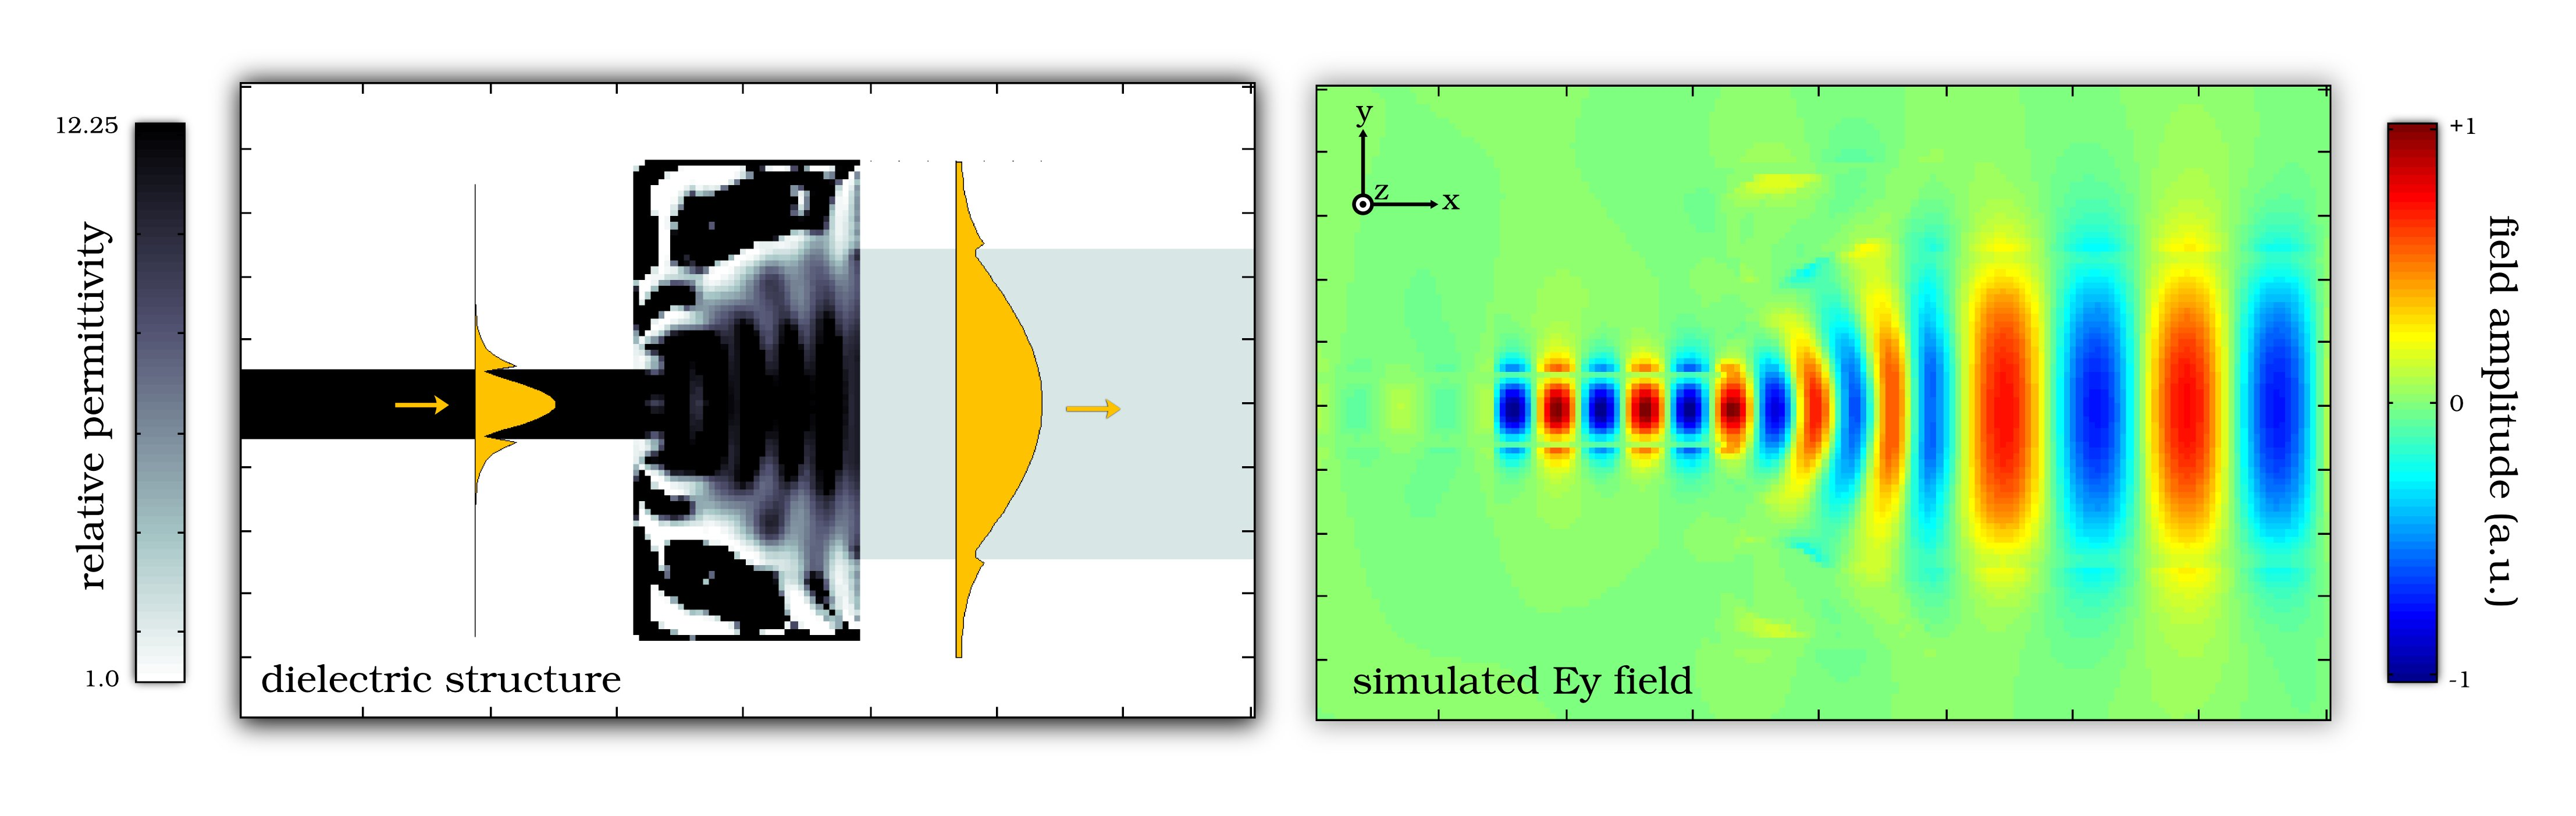
\includegraphics[width=0.9\textwidth]{fig/fiber.jpg}
%     \caption{Waveguide coupler for a wide, low-index waveguide. 
%         The dielectric structure of the coupler and surrounding input and
%         output waveguides is shown on the left, while the simulation
%         validating our results is shown on the right.
%         The coupler converts $96.3\%$ of the input power to the
%         designated output mode.
%         The device is extremely compact, 
%         convering only $36 \times 66$ grid points,
%         where the vacuum wavelength is 42 grid points.
%         Computation time was 20 minutes on a personal computer.}
% \end{figure}
% \begin{figure}[htbp]
%     \centering
%     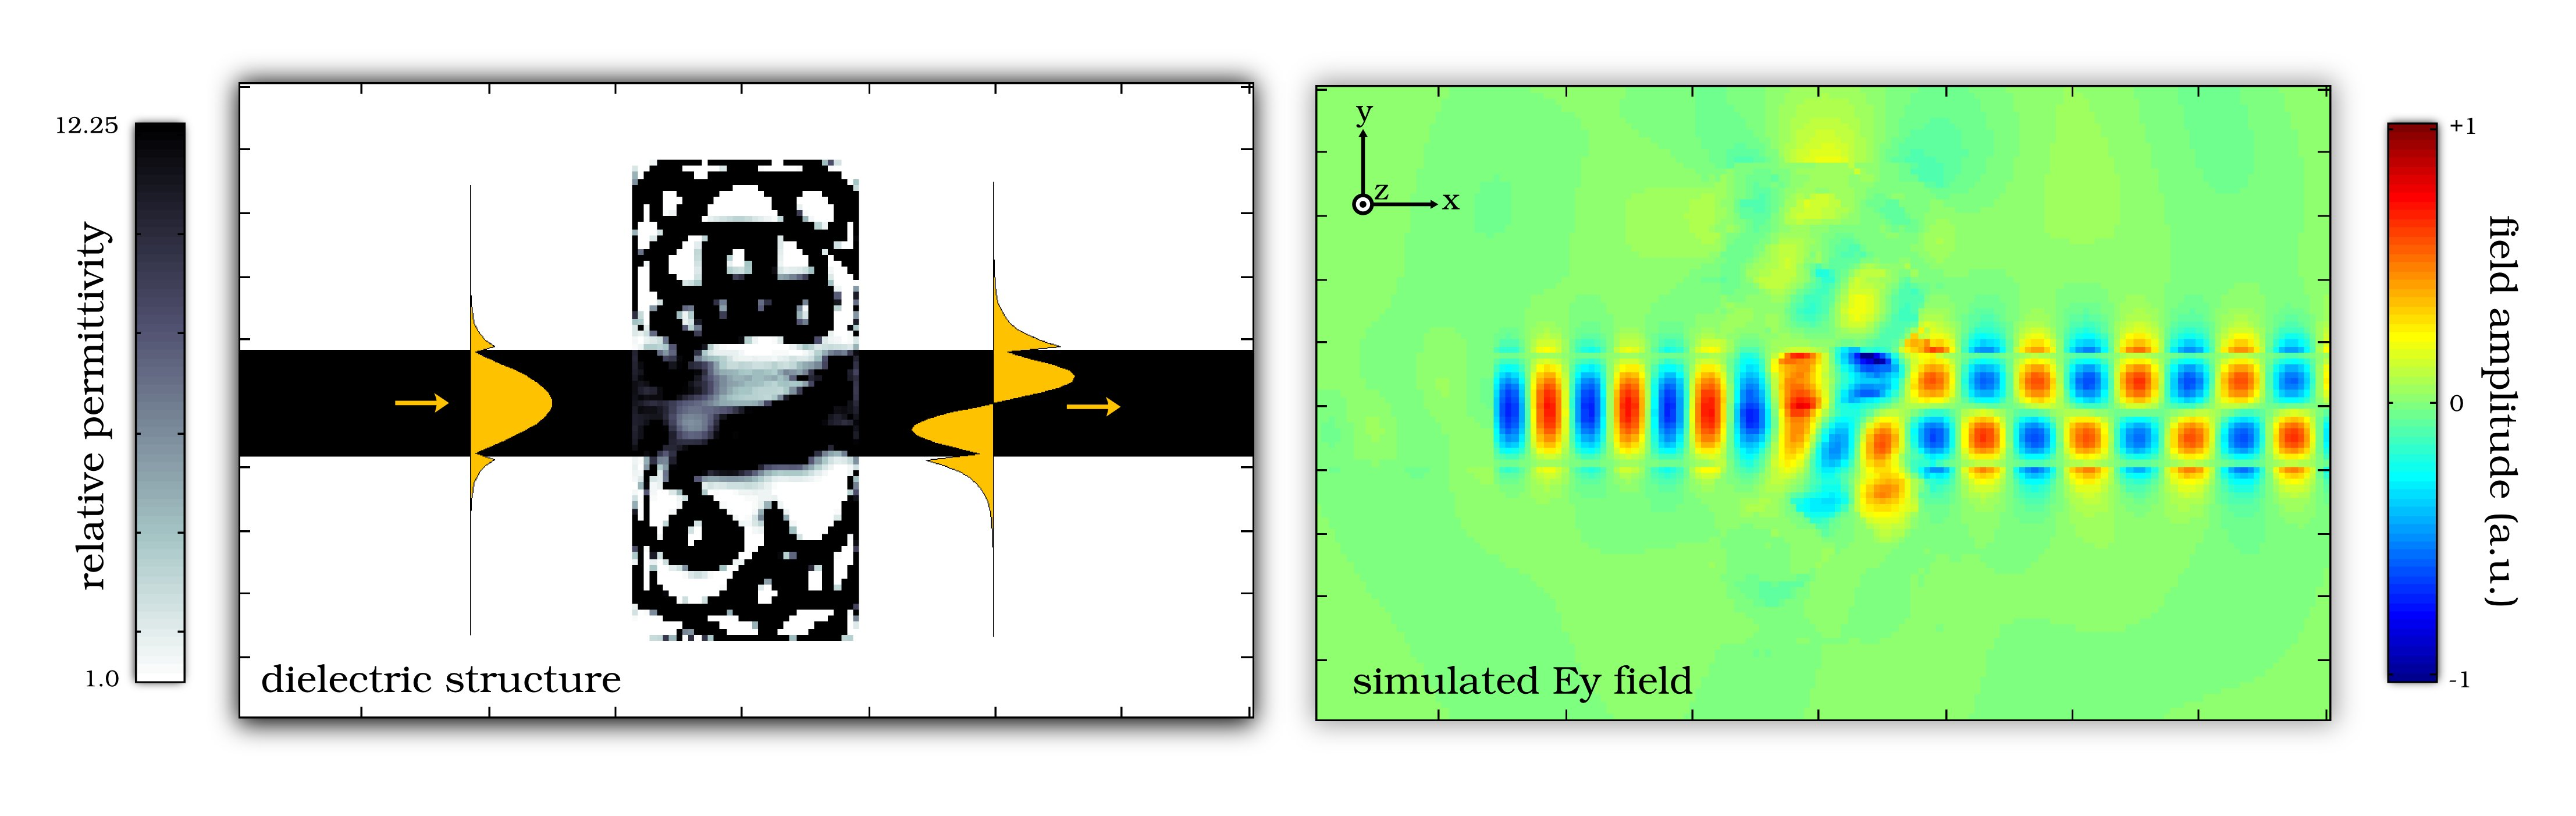
\includegraphics[width=0.9\textwidth]{fig/mode-conv.jpg}
%     \caption{Coupler that converts the fundamental waveguide mode to the
%         second-order waveguide mode.
%         This problem is quite difficult since the two modes are of 
%         opposite symmetry.
%         For example, adiabatic approaches cannot be applied to this case.
%         However, our method produces a device 
%         (which has the same dimensions and vacuum wavelength as Fig. 1) 
%         which achieves a coupling efficiency of $95.5\%$. 
%         Computation time was extended to 50 minutes to improve efficiency.
%         }
% \end{figure}
% \begin{figure}[htbp]
%     \centering
%     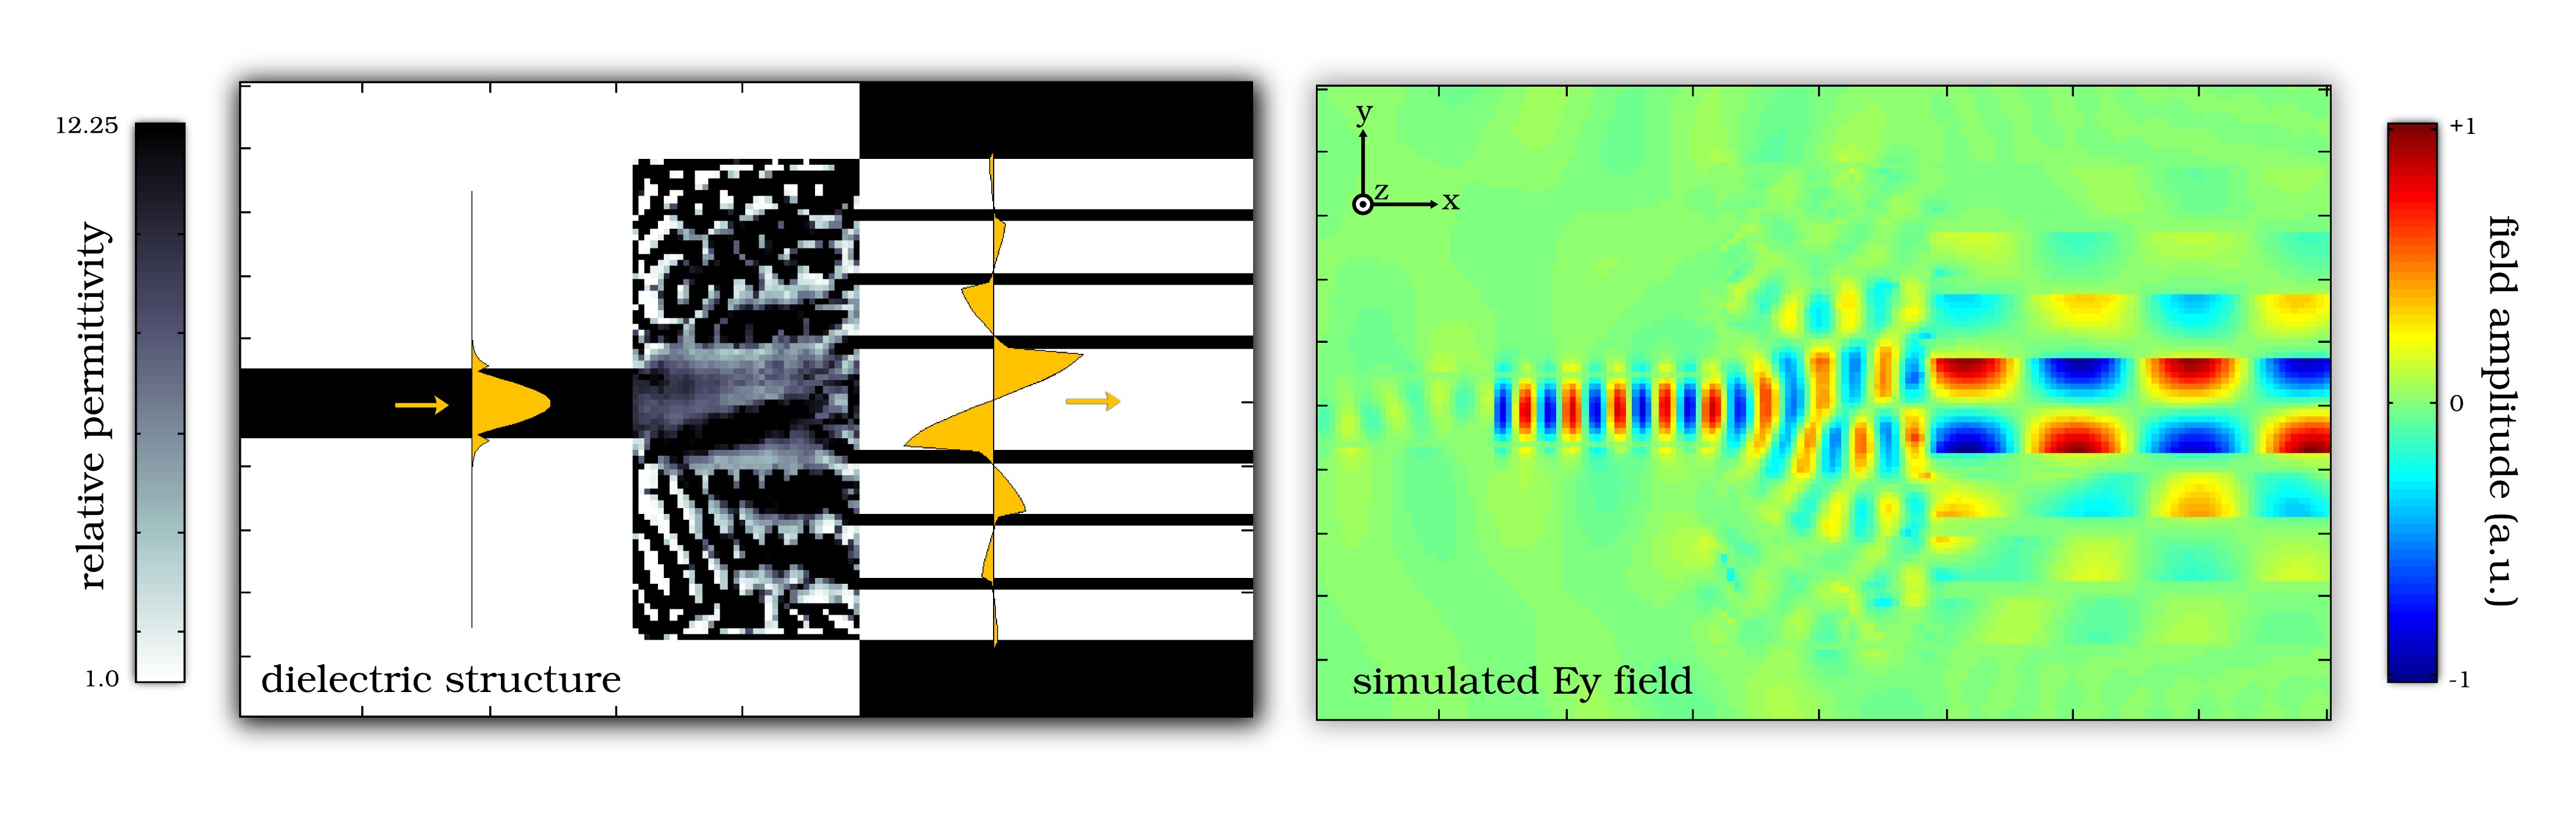
\includegraphics[width=0.9\textwidth]{fig/air-core.jpg}
%     \caption{Coupler to an air-core mode.
%         Here, not only are the modes of opposite symmetry,
%         but the output waveguide operates on a fundamentally different
%         principle (guided by Bragg reflection) than the input waveguide 
%         (index guided).
%         The device still achieves an efficiency of $83.3\%$, demonstrating the
%         versatility of our method.
%         The vacuum wavelength is 25 grid points, 
%         while the device footprint is still $36 \times 66$ grid points.
%         Computation time was 20 minutes.
%         }
% \end{figure}

\end{document}

